\begin{Example}[vietnam1]{Student opinion about the Vietnam war}
In May 1967 a survey of student opinion on U.S. policies toward the war in Vietnam was undertaken at the University of North Carolina at Chapel Hill.
Students were asked which of four policies they supported.  The alternatives stated that the US should \dots:
\begin{description*}
\item[A] defeat North Vietnam by widespread bombing and by land invasion.
\item[B] follow the present policy.
\item[C] de-escalate military activity, stop bombing, and intensify efforts to begin negotiations.
\item[D] withdraw military forces immediately.
\end{description*}
The responses were classified by gender and by student status (undergraduate year, or graduate student),  published in the student newspaper, and subsequently analyzed by \citet{Aitkin-etal:89}.  The data are shown in
\tabref{tab:vietnam1} and listed in the \Dset\ \pname{VIETNAM}
in \datref{dat:vietnam}.
\begin{table}[htb]
 \caption{Student opionion on Vietnam war policy}\label{tab:vietnam1}
 \begin{center}
 \begin{tabular}{ll rrrr rrr}
  \hline
       &       &  \multicolumn{4}{c}{Response} \\ \cline{3-6}
Sex    & Year  &   A  &  B  &  C  &  D  & Total & Enroll & \% Resp \\ \hline
Male   & 1     &  175 & 116 & 131 &  17 & 439 & 1768 & 24.8 \\ 
       & 2     &  160 & 126 & 135 &  21 & 442 & 1792 & 24.7 \\ 
       & 3     &  132 & 120 & 154 &  29 & 435 & 1693 & 25.7 \\ 
       & 4     &  145 &  95 & 185 &  44 & 469 & 1522 & 30.8 \\ 
       & Grad  &  118 & 176 & 345 & 141 & 780 & 3005 & 26.0 \\[.5ex] 
Female & 1     &   13 &  19 &  40 &   5 &  77 &  487 & 15.8 \\ 
       & 2     &    5 &   9 &  33 &   3 &  50 &  326 & 15.3 \\ 
       & 3     &   22 &  29 & 110 &   6 & 167 &  772 & 21.6 \\ 
       & 4     &   12 &  21 &  58 &  10 & 101 &  608 & 16.6 \\ 
       & Grad  &   19 &  27 & 128 &  13 & 187 & 1221 & 15.3 \\ 
  \hline
 \end{tabular}
 \end{center}
\end{table}


The survey was not designed to yield a representative sample
(survey ballots were merely made available in the student council building)
and the response rates, shown in \tabref{tab:vietnam1}, were low overall
and varied somewhat according to year and gender.
We cannot, therefore, draw conclusions about the attitudes of the whole student population.
However, we can study how the preferred policy varies with sex and year of study, among those who responded.
This means that the total numbers of each sex and year should be regarded
as fixed, and the [SexYear] term must be included in any model.
Note that both the response and year might reasonably be treated as ordinal
variables.

The \Dset\ \pname{vietnam}, listed in \datref{dat:vietnam}, is created in frequency form
with the variables \pname{sex}, \pname{year}, \pname{response}, and
\pname{count}.  Both \pname{year} and \pname{response} are created as
numeric variables to allow them to be treated as ordinal (or interval)
variables, and formats are created to associate descriptive labels
as needed.

Because response choice is the natural outcome variable, it is useful
to begin with a simple graph showing the proportions of choices
for each Sex-Year group, shown in \figref{fig:vietprob}.
%% two subfig side-by-side
\begin{figure}[htb]
 \begin{minipage}[t]{.49\linewidth}
  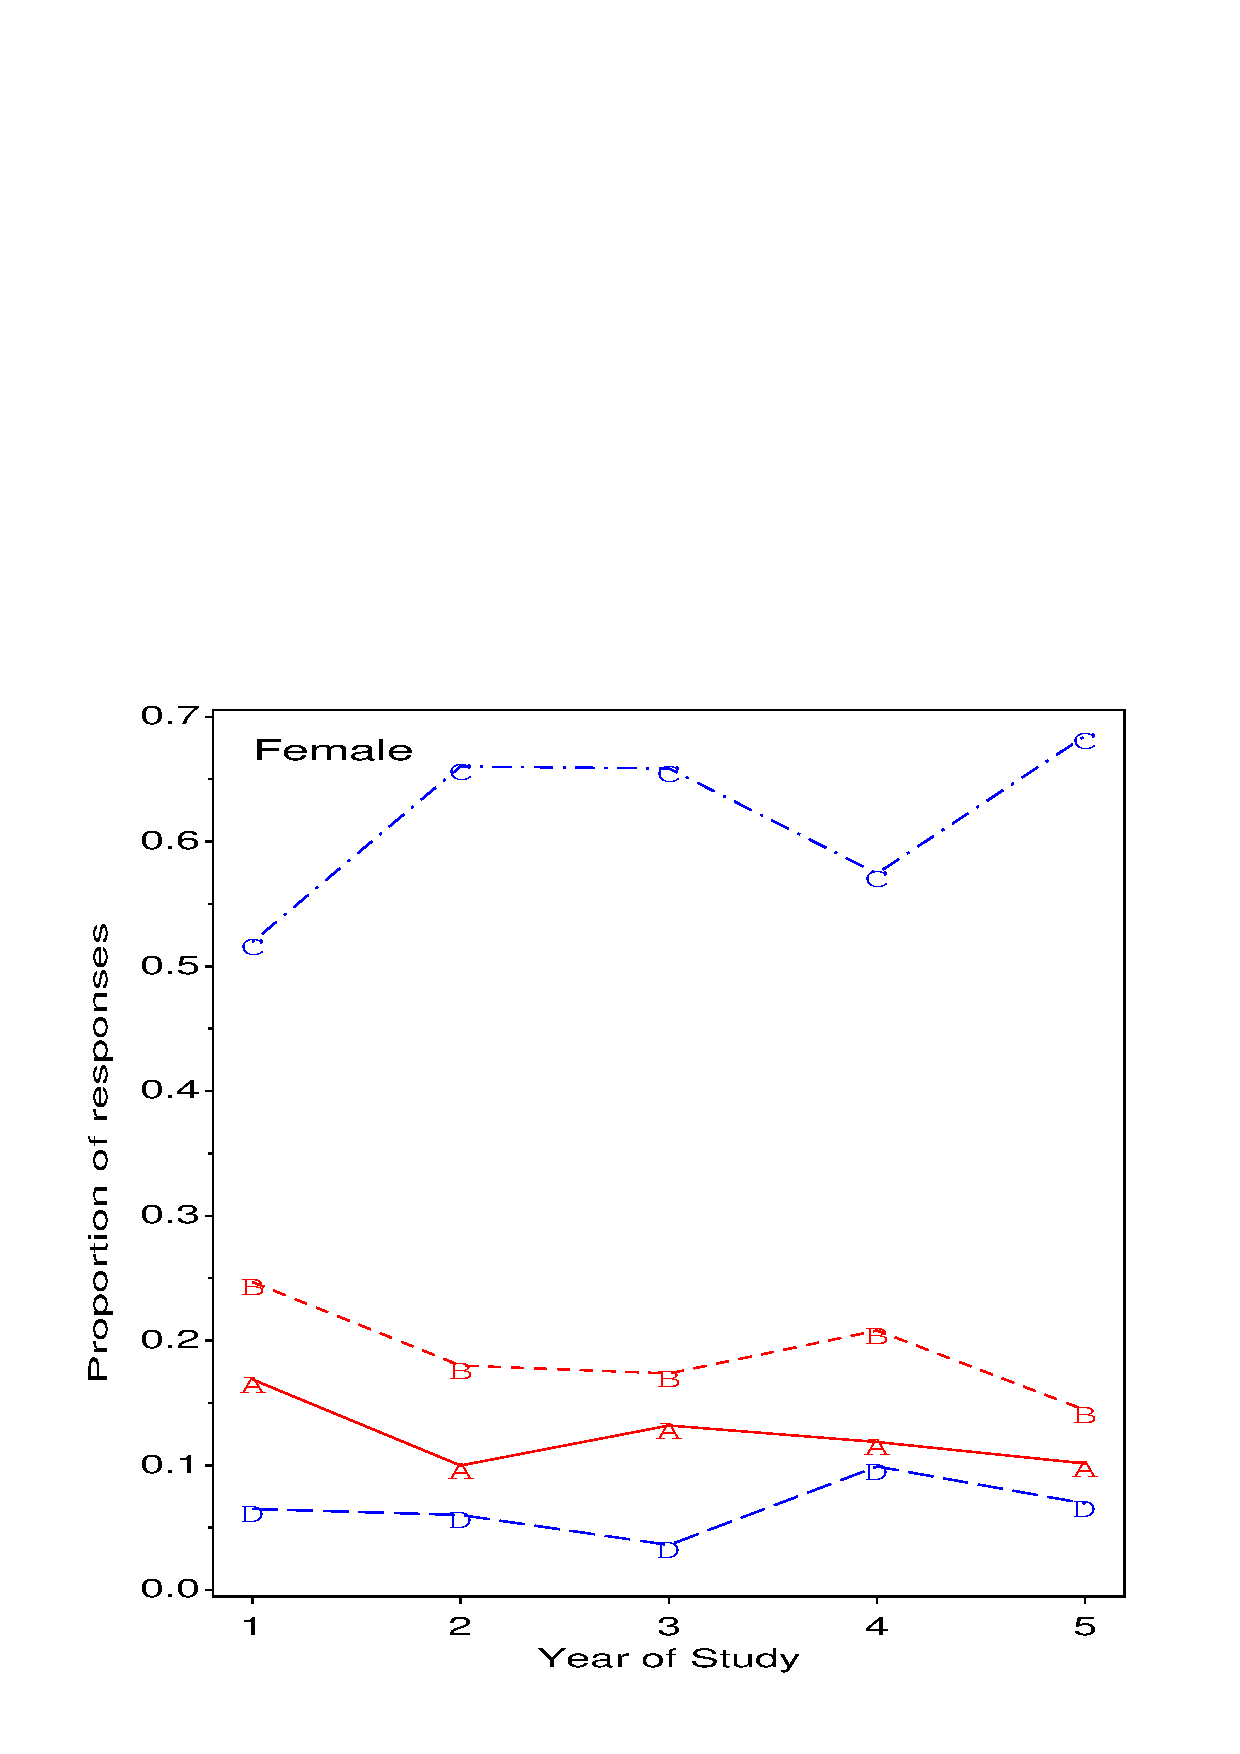
\includegraphics[width=1\linewidth]{vietprob1}
 \end{minipage}%
 \hfill
 \begin{minipage}[t]{.49\linewidth}
  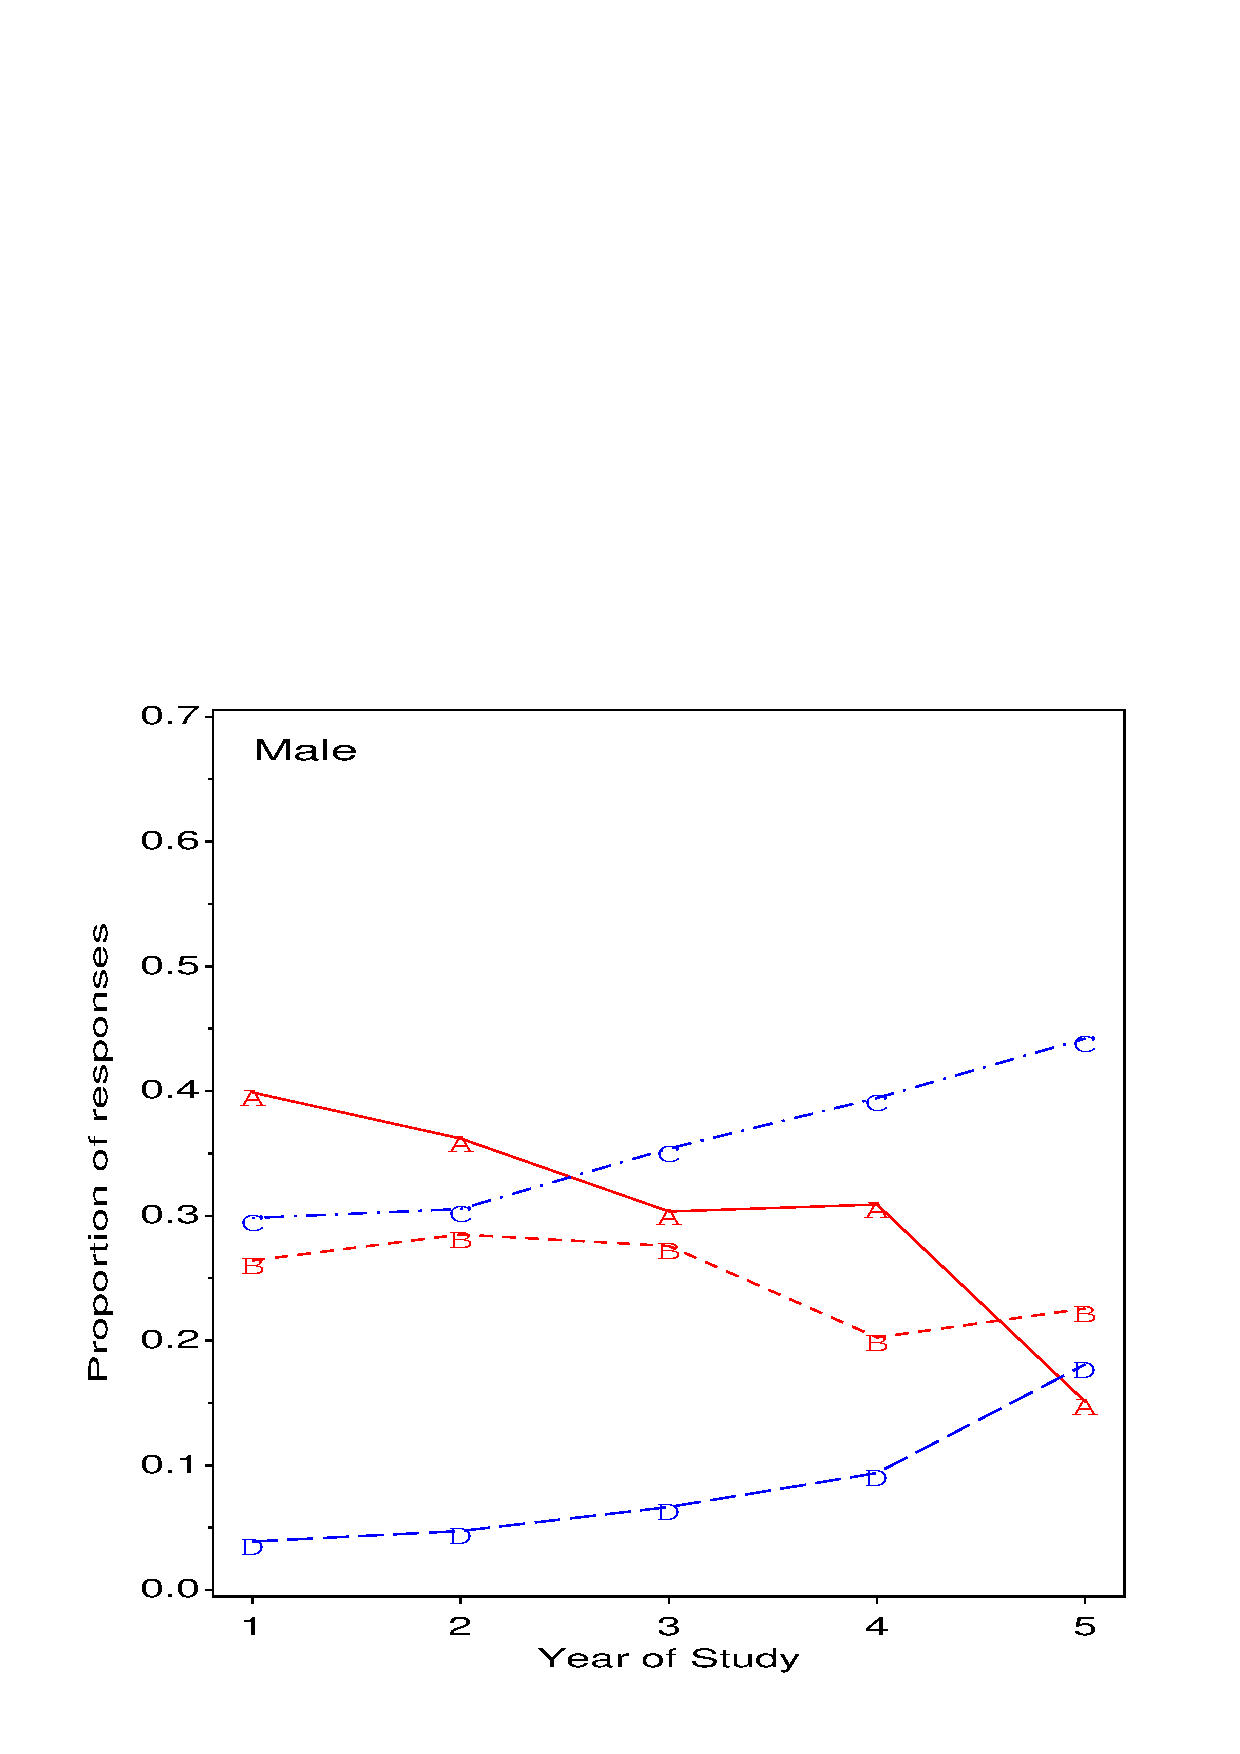
\includegraphics[width=1\linewidth]{vietprob2}
 \end{minipage}
 \caption[Response probabilities for Vietnam data]{Response probabilities for Vietnam data.  Point labels indicate the response category.}\label{fig:vietprob}
\end{figure}
To do this, we find the total number of respondents in each group,
merge this with the data, and calculate the proportions.
%% input: /users/faculty/friendly/sasuser/catdata/vietprob.sas
%% last modified: 23-Oct-98  9:38
\begin{listing}
%include catdata(vietnam);

*-- Get row totals for sex-year;
proc summary data=vietnam nway;
   class sex year;
   var count;
   output out=totals sum=total;

*-- Merge, compute proportions;
data vietnam;
   merge vietnam totals(keep=sex year total);
   by sex year;
   p = count / total;
   label p='Proportion of responses';
\end{listing}

Then, we can plot \pname{p} against \pname{year} for each \pname{sex},
giving the graphs shown in \figref{fig:vietprob}:
%% input: /users/faculty/friendly/sasuser/catdata/vietprob.sas
%% last modified: 23-Oct-98  9:38
\begin{listing}
goptions hby=0;
proc gplot data=vietnam;
   plot p * year = response / 
      frame vaxis=axis1 haxis=axis2 hm=0 vm=1 nolegend anno=label;
   by sex;
   symbol1 v=A h=2 i=join c=red  l=1;
   symbol2 v=B h=2 i=join c=red  l=20;
   symbol3 v=C h=2 i=join c=blue l=41;
   symbol4 v=D h=2 i=join c=blue l=21;
   axis1 label=(a=90) order=(0 to .7 by .1);
   axis2 offset=(3);
\end{listing}


From these graphs, we see that women choose response C, ``begin negotiations''
most often, and the ranking of their choices is relatively
constant over years.
For men, however, the proportions choosing ``doveish'' responses C and D increase
consistently over years, while the proportions for A and B decrease.
We keep these observations in mind as we begin to search for a descriptive model.

We begin by fitting the baseline ``null'' model, $[SY][R]$, which includes the
$[SY]$ association, but no association between response and sex or year.
This model implies that the response curves in \figref{fig:vietprob}
should all be flat (no year effect) and at the same levels in the two
panels (no sex effect).
The model fit is very poor ($G^2$ (27) = 361.72), and the patterns in
\figref{fig:vietprob} lead us to add sex and year effects, giving
the model $[SY][RS][RY]$.
These two models are fit using \PROC{CATMOD} using the
\stmt{LOGLIN}{CATMOD} as follows:
%% input: /users/faculty/friendly/sasuser/catdata/vietnam1.sas
%% last modified: 23-Oct-98  9:59
\begin{listing}
*-- Fit as loglin models;
proc catmod data=vietnam;
   weight count;
   model response * sex * year = _response_ /
         ml noiter noresponse nodesign nogls noprofile;
   loglin response sex|year / title='Null model';
 run;
   loglin sex|year response|sex response|year / title='Sex+Year';
 run;
\end{listing}


The model summary statistics from this step are shown in
\outref{out:vietnam1.1}.  For the second model, the
$[RS]$ and $[RY]$ terms are both large, and the model
fit is dramatically improved.
Given the large sample size, we might accept this as
an adequate model, particularly if we had not plotted the data.

\begin{Output}[htb]
\caption{Model fit summaries for initial models, Vietnam war data}\label{out:vietnam1.1}
\small
\verbatiminput{ch7/out/vietnam1.1}
\end{Output}

%% two subfig side-by-side
\begin{figure}[htb]
 \begin{minipage}[t]{.49\linewidth}
  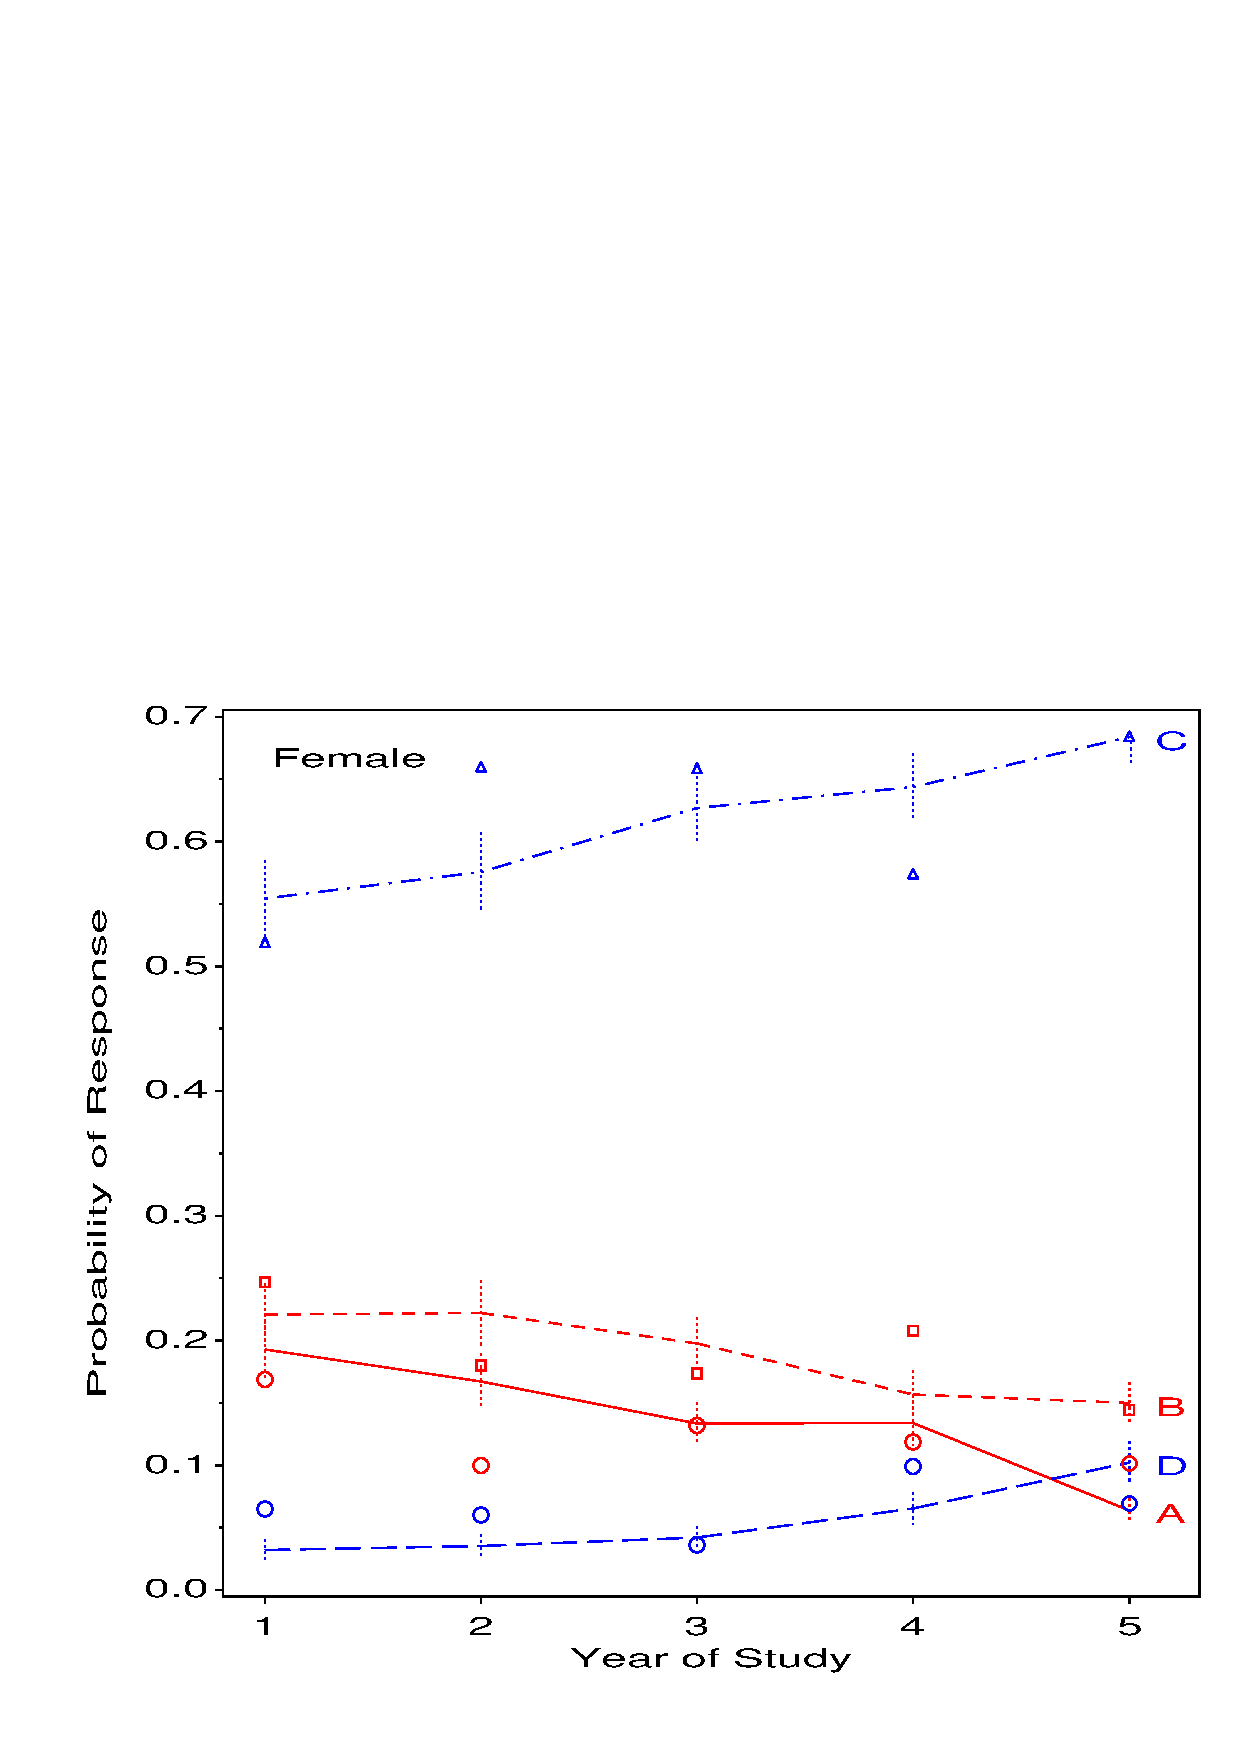
\includegraphics[width=1\linewidth]{vietnam11}
 \end{minipage}%
 \hfill
 \begin{minipage}[t]{.49\linewidth}
  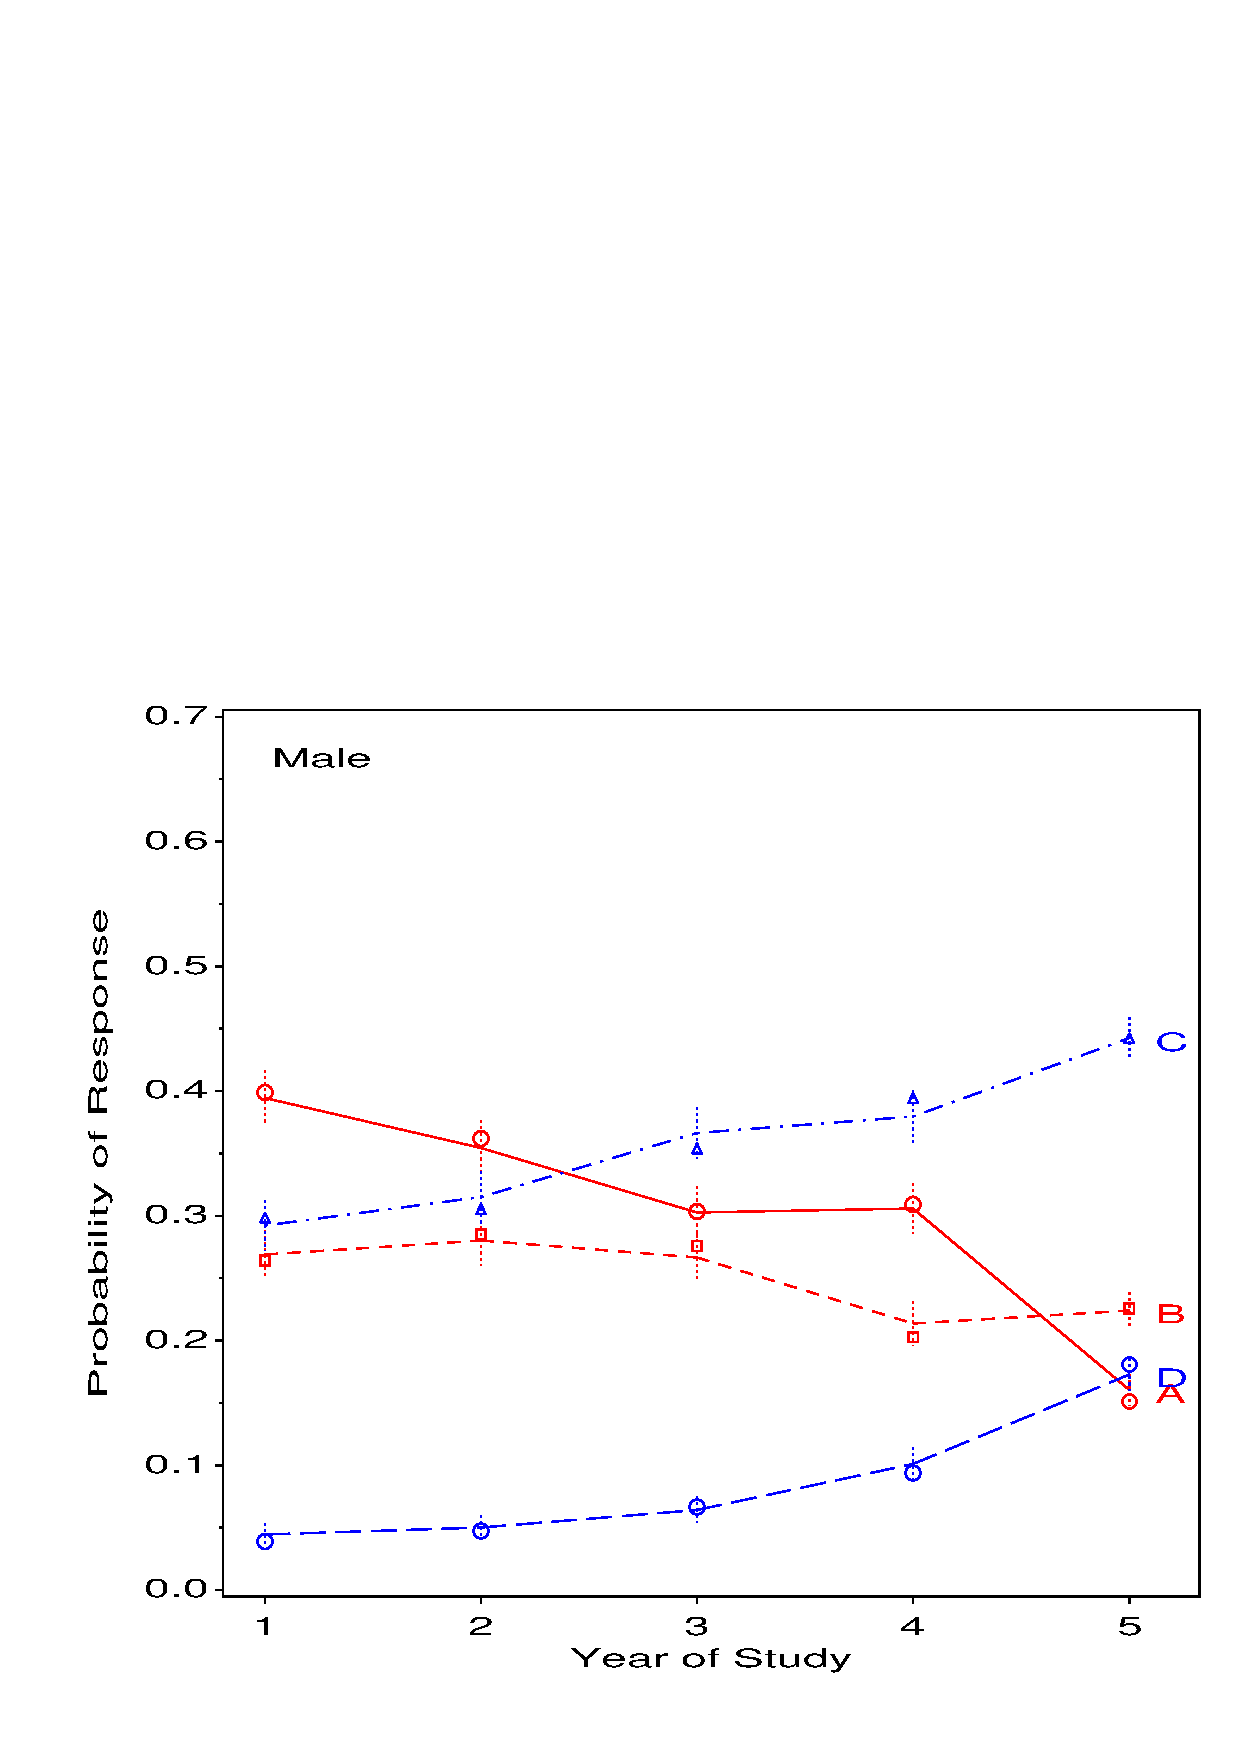
\includegraphics[width=1\linewidth]{vietnam12}
 \end{minipage}
 \caption{Observed and fitted probabilities for model $[SY][RS][RY]$}\label{fig:vietnam1}
\end{figure}

The \LR\ \GSQ\ for the Sex+Year model, 19.19 on 12 df, corresponds to the three-way
term, $[RSY]$.  Excluding it from the model means that the
relationship between response and year is the same for men and
women, yet we have seen in \figref{fig:vietprob} that this
is unlikely to be true.  There is something wrong with the Sex+Year
model.

We can confirm these suspicions by plotting predicted probabilities
under the model together with the observed response probabilities.
For a \loglin\ model,
\PROC{CATMOD} gives fitted \emph{frequencies}, and we could divide these
by the totals as we did to produce \figref{fig:vietprob}.
It is somewhat easier to fit the equivalent logit model for \pname{response},
for which the fitted values (with \verb|_TYPE_='PROB'| in the \ODS) are probabilities.
The \macro{CATPLOT} produces \figref{fig:vietnam1}.
%% input: /users/faculty/friendly/sasuser/catdata/vietnam1.sas
%% last modified: 23-Oct-98  9:59
\begin{listing}
*-- Fit as logit models;
proc catmod data=vietnam;
   weight count;
   population sex year;
   response logit;
   model response = / ml noiter noprofile title='Null model';
 run;
   response logit / out=fit;
   model response = sex year/ ml noiter noprofile title='Sex+Year';
 run;

axis1 label=(a=90) order=(0 to .7 by .1);
axis2 offset=(3,5);
%catplot(data=fit,
   x=year, y=_obs_,
   type=PROB,
   class=response, clfmt=letter.,
   byvar=sex, byfmt=$sex.,
   vaxis=axis1, haxis=axis2,
   colors=red red blue blue,
   ylab=Probability of Response);
\end{listing}


The fitted probabilities are reasonably close for males, but quite poor for females.  Perhaps we need to fit different models for men and women.
The saturated \loglin\ model, $[RSY]$ corresponds to the logit model
$R = S | Y = S + Y + S*Y$.
We can examine the possibility of different year effects for men and women within the logit formulation by nesting the effect of year within sex.
(This is equivalent to fitting separate models, $R = Y$, by sex.)
%% input: /users/faculty/friendly/sasuser/catdata/vietnam1.sas
%% last modified: 20-Nov-98  9:49
\begin{listing}
*-- Year within Sex;
proc catmod data=vietnam;
   weight count;
   population sex year;
   model response = sex  year(sex='F')  year(sex='M')
     / ml noiter noprofile title='Year within Sex';
   response logit ;
\end{listing}


The output, shown in \outref{out:vietnam1.2}, indicates that the year
effect for women is quite small ($\GSQ(12) = 12.96$) and can be dropped
from the model.
Removing the term \pname{year(sex='F')} from the \pname{model} statement
gives an adequate model;
the residual $\GSQ(12) = 12.96$ in the revised model
is (coincidently) just that for the term dropped.
\begin{Output}[htb]
\caption{Vietnam war data, Nested year effect model}\label{out:vietnam1.2}
\small
\verbatiminput{ch7/out/vietnam1.2}
\end{Output}

We noticed earlier that the response probabilities for men were consistently
increasing or decreasing with year.  Perhaps we can simplify the model
by using year as a linear effect.  To do this, we just add the statement
\pname{DIRECT YEAR;}.
%% input: /users/faculty/friendly/sasuser/catdata/vietnam2.sas
%% last modified: 20-Nov-98 11:05
\begin{listing}
*-- Year-linear within Males;
proc catmod data=vietnam;
   weight count;
   population sex year;
   direct year;
   model response = sex year(sex='M')
       / ml noiter noprofile title='Year-linear within Males';
   response / out=fit;
\end{listing}


The model fit statistics for this model (\outref{out:vietnam2.1})
suggests there is some lack-of-fit, however, with $\GSQ (21) = 38.10$.
To see why, plot the observed and fitted probabilities again.
Because the plot is determined completely by the \ODS\ \pname{fit},
we use exactly the same \pname{\%catplot} call as for \figref{fig:vietnam1}.
The result is shown in \figref{fig:vietnam2}.
\begin{Output}[htb]
\caption{Vietnam war data, Linear year effect for males}\label{out:vietnam2.1}
\small
\verbatiminput{ch7/out/vietnam2.1}
\end{Output}

Most of the observed points in \figref{fig:vietnam2} are quite close to
the fitted values (the error bars show $\pm 1$ standard error
around the predicted probability). However, there are a few scattered points for
females and a couple for males (4th year, responses A and B) which appear poorly fit.

We should certainly examine residuals more closely
to see if the lack-of-fit is localized to these few cells
or whether there is a more general way to improve the model.
For example,  the two points for 4th year men
indicate a tendency for them to select response B less than the model predicts, and to select
response A more often.
 \citet{Aitkin-etal:89} make the reasonable
suggestion that these draft-eligible men would eschew the ``present policy''
under which their chances of being drafted would increase.
But perhaps it's time to look at these data from another perspective.

%% two subfig side-by-side
\begin{figure}[htb]
 \begin{minipage}[t]{.49\linewidth}
  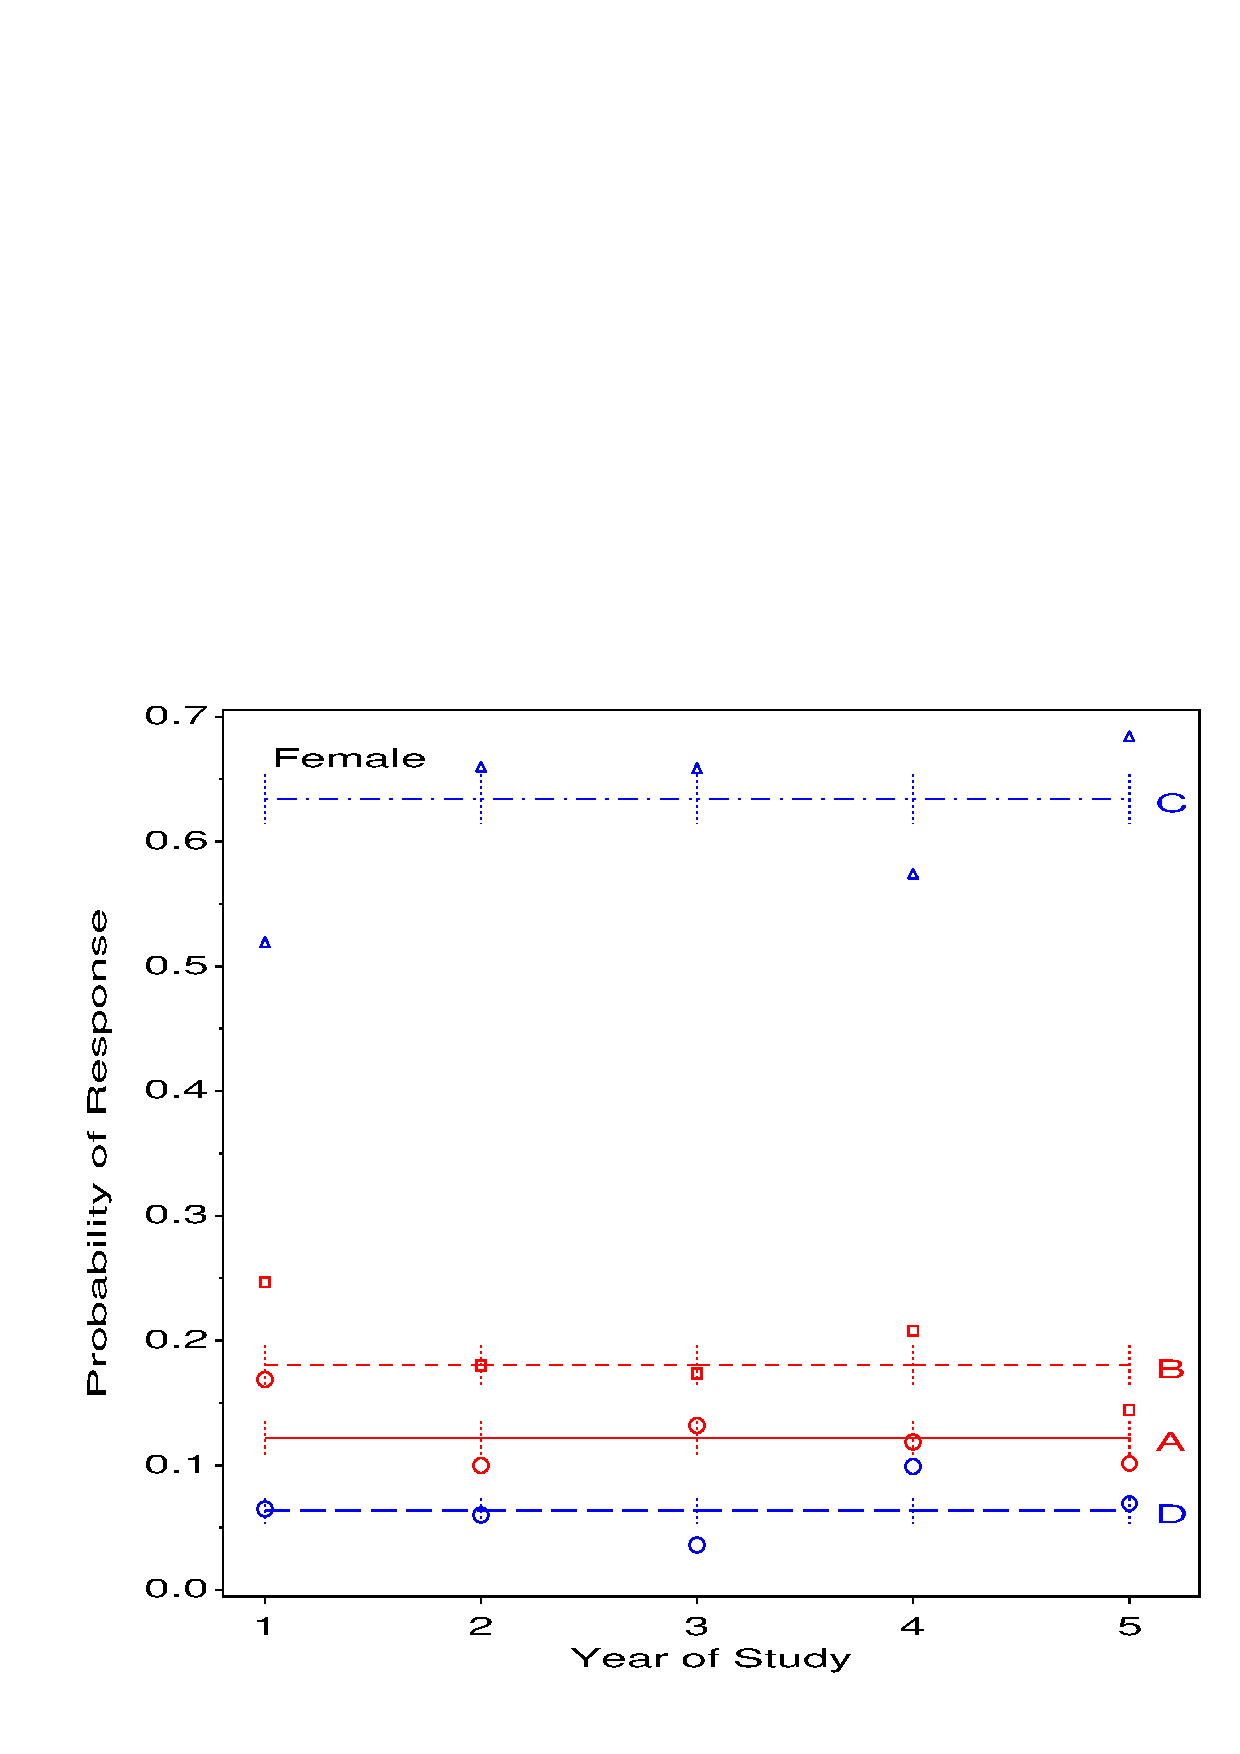
\includegraphics[width=1\linewidth]{vietnam21}
 \end{minipage}%
 \hfill
 \begin{minipage}[t]{.49\linewidth}
  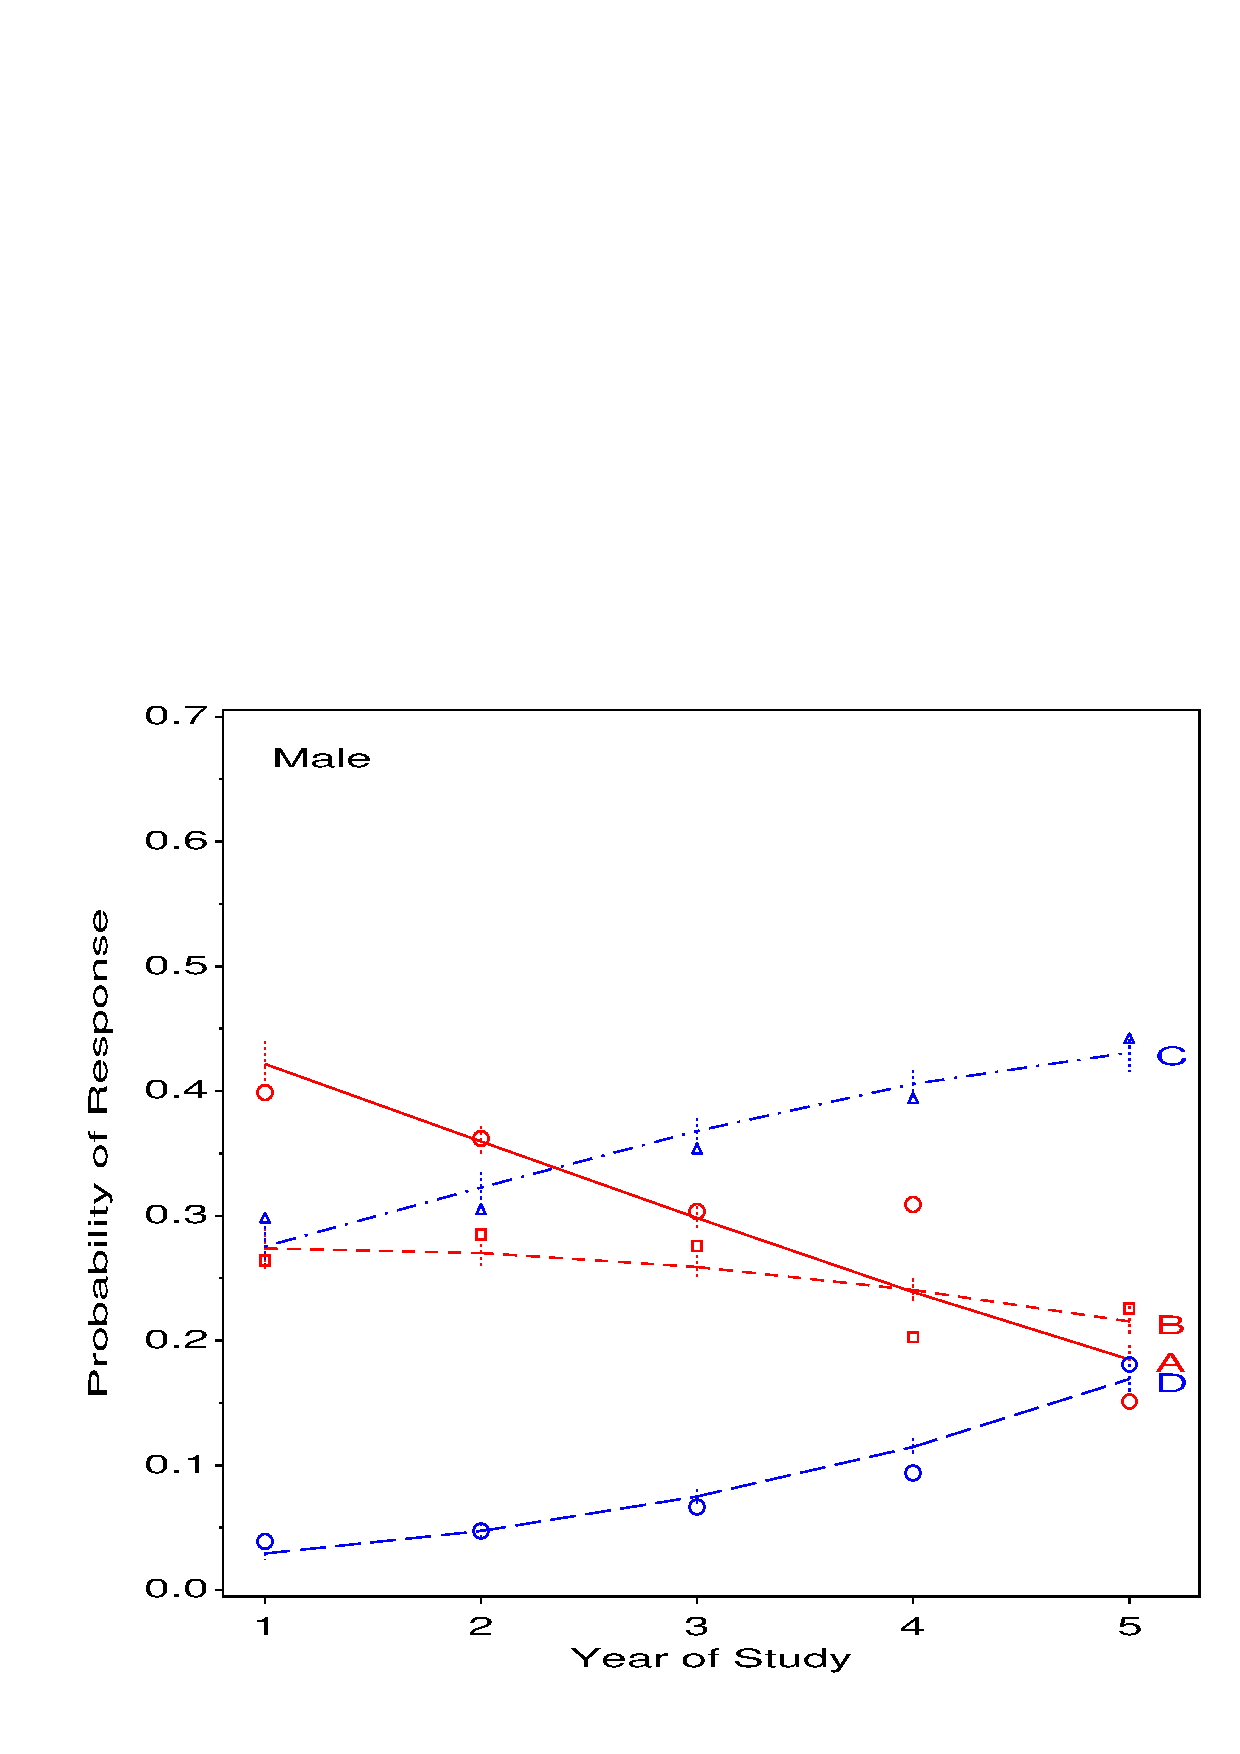
\includegraphics[width=1\linewidth]{vietnam22}
 \end{minipage}
 \caption{Observed and fitted probabilities for model $R = S + Y_{lin}(M)$}\label{fig:vietnam2}
\end{figure}
\end{Example}
